\begin{figure}%
	\centering%
	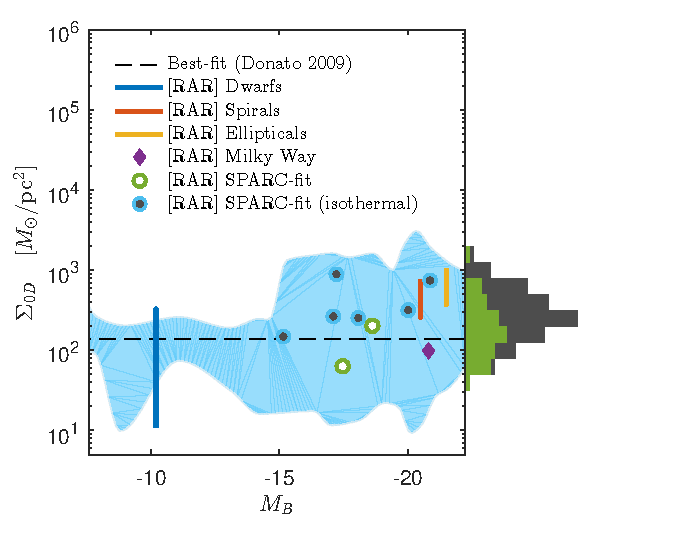
\includegraphics[width=\hsize]{\ROOTPATH/fig.pdf}
	\caption{DM surface density ($\Sigma_{0D}$) predictions in the fermionic model using the SPARC data-set. The blue region indicates the delimited area by the $3\sigma$ error bars of all the data points in \citet{2009MNRAS.397.1169D}. The violet diamond represents the MW as analyzed in \cite{2018PDU....21...82A}. The absolute magnitude was taken from the Carnegie-Irvine Galaxy Survey \citep{2011ApJS..197...21H}, providing nine overlapping galaxies (blue and green circles). The full  sample (gray bars) and sub-sample (green bars) including only for non-isothermal solutions ($W_p < 10$), are shown as histograms, both following approximately a Gaussian distribution.}%
	\label{fig:SPARC:Donato}%
\end{figure}